\documentclass[10pt]{article}
\usepackage[margin=0.75in]{geometry}
\usepackage{amsmath,amssymb,amsfonts,cancel}
\usepackage{verbatim}
\usepackage{float}
\usepackage{tikz, pgfplots}
\usetikzlibrary{external}%makes separate image
\tikzexternalize[only named, optimize=false,shell escape=-shell-escape]
\usetikzlibrary{arrows,decorations.pathmorphing,backgrounds,positioning,fit}
\usetikzlibrary{petri,intersections,calc,through,decorations.markings}
\usepackage{pgfplotstable}
\pgfplotsset{compat=1.8}

\title{Guess Your Hat Color, A Brain Teaser}
\author{Owen M. Dix}
\date{}
\begin{document}

\maketitle

Here is the riddle as I've heard it. One hundred captives are being held in 
one area of a Nazi concentration camp, and the Nazi warden decides to play a 
particularly cruel game. He gives these captives 24 hours to come up with 
a plan to solve this game, and their lives are on the line. In 24 hours 
time, each of the captives will have placed on his/her head a hat
colored entirely in either red, green, or blue. Which 
of the three colored hats is used for a person may be entirely random. To 
survive this game, each person must guess the hat color on their own head. 

The 100 captives 
will be lined up in random order in a straight, single-file line, 
facing the back of the person in front of them. Then the hats will be placed 
on their heads.
They are not allowed to see the color of the hat ahead of time, and if they 
try to peek at their own color, they will be shot. They are allowed to 
talk only to say their own hat color. Any other utterances will
get that person killed. They are allowed to look around but not 
face backwards since seeing the person behind them could easily 
allow for some form of communication beyond shouting out their 
own hat color. Leaning left or right is okay so the captives will be able to 
see the hats of all people in front of them, but since they cannot turn 
around, they won't be able to silently communicate this. Accept this as a
given. After the hats get placed on their heads they can take their time 
to answer, but the person in back will answer first and the guards will 
work their way up to the front of the line, to the person who cannot see 
anybody's hat. If evidence is found that any of the 100 captives is cheating, 
trying to communicating verbally or nonverbally - even 
by patterns in their inflection - in any other way 
than shouting their own hat color out to the warden, everyone will be killed.

Clearly actually doing this would be horrible,
but this does make an interesting brain teaser. Your goal is to 
find the strategy that, on average, would lead to the highest number of 
survivors, without cheating.

\section{Hints}

\begin{itemize}
    \item Don't try to find a secret way to communicate information, 
    outside of the hat color each person shouts in order. Other forms 
    of communication are considered cheating and spoil the fun.

    \item Just guessing would lead to an average of $33\tfrac{1}{3}$ 
    survivors out of the original 100.

    \item If performed flawlessly, the optimal strategy
    would lead to an average of $99\tfrac{1}{3}$ survivors.
\end{itemize}

Spoilers: the next hints are encoded, and can be read one-by-one for 
incremental help.

\begin{itemize}
    \item (Read two words, skip one, repeat.) 
        As far and as I people know, you eat will need people some math 
        hats concepts to undo solve this juggalo problem.
    
    \item (Read two words, skip one, repeat.)
        All information complexity about what person hat 
        someone too is wearing can must come with
        from the answer guesses of time the people ahead
        before them, time using what simpler they can fourth
        see ahead strategy of them, but and knowledge conceptualize
        of the concentration code.

    \item (Read every other word, starting with the second.) 
        Stop assign mothers a happy number until to 
        over each concentration hat captives color, head the most simplest will 
        being alpha zero, beta one, gamma and delta two echo.

    \item (Read every other word, starting with the third.)
        Games form everyone tries sums hundred the easily hat math colors 
        peek in person front shot of communicate them inflection.

    \item (Read every other word, starting with the fourth.)
        Jewish camp cannot the single first line guesser from gets are no 
        they information blue so of they a should I guess you
        the an sum if of for all to hat alpha 
        colors time in on front with of beyond 
        them able as hear their all own in hat face. How why?

    \item (Read two words, skip one, repeat.)
        All sums take can be undone mapped into treasure the three bears 
        numbers if sneeze you take front the remainder color of the 
        trying sum when multiply divided by alpha three. Information shout 
        is preserved average but you interest need to see work out headed 
        what calculation than everyone must than make.
        
\end{itemize}

\newpage

\section{Solution}

The captives define the following mapping:
\begin{align*}
    \text{red} &= 0 \\
    \text{green} &= 1 \\
    \text{blue} &= 2
\end{align*}
Note that the colors are ascending in number in roygbiv order, to 
make it easier to remember how to map the number back to the colors. 
Each person will have a hat value for their own head. They will 
do some math, get a number (either 0, 1, or 2), and map that back to 
the appropriate color above to yell it out as their guess. 
The $i$-th person's 
hat value is symbolized as $h_i$:
\begin{equation*}
    h_i \in \mathbb{Z}_3 = \{0,1,2\}
\end{equation*}
Here $\mathbb{Z}_3$ is the cyclic group of non-negative 
integers less than 3, which is just the set of numbers 0, 1, and 2. $\in$ 
means ``is an element of''. So this equation says: ``the hat numbers can only 
take on the values 0, 1, and 2''. The 
index, $i$ will start from the back of the line and work towards the 
front. Because each person may not guess their hat correctly, we should 
also define $g_i$, the guess value for the $i$-th person. Clearly, if they 
don't guess their actual hat value (mapped back to the colors), then they will 
die:
\begin{align*}
    g_i &= h_i \Rightarrow\text{live} \\
    g_i &\neq h_i \Rightarrow\text{die}
\end{align*}
Finally, the key to surviving is to use the modulo-3 function: take the 
remainder of a number when you divide it by 3. This function will always 
return a number within the cyclic group $\mathbb{Z}_3$, so it can be mapped 
to one of the three colors. This is commonly symbolized with the 
\% operator, e.g.
\begin{align*}
    0\%3&=0 \\
    1\%3&=1 \\
    2\%3&=2 \\
    3\%3&=0 \\
    4\%3&=1 \\
    5\%3&=2 \\
    6\%3&=0 \\
    7\%3&=1 \\
    \ldots
\end{align*}
We will now need to define the 
modulo-3 of the sum of all hat values 
in front of person $i$, as:
\begin{equation*}
    s_i = \left(\sum_{j=i+1}^{100} h_j\right)_{\mathbb{Z}_3}
        = \left(\sum_{j=i+1}^{100} h_j\right) \% 3
\end{equation*}
This says taking the modulo-3 is the same as doing all your math in the 
cyclic group $\mathbb{Z}_3$. See the Appendix for details on 
how to use this sort of math. 
Once this is defined, and we establish a rule that everyone knows, 
everyone not in the very back will have the information needed to 
calculate their own hat value then map it back to the colors. 
We have 
to first establish the rule, that everyone has to know, for what the first 
person in the back will do, since they have no information. 
The person in the very back will guess the value they calculate for $s_{i=1}$, 
the modulo-3 of the sum of all hat values in front of them. Notice I am starting 
my index numbering from 1, not 0 like computer scientists often like.
\begin{equation*}
    g_1 = s_1
\end{equation*}
The person in the very back will have a $1/3$ chance of guessing their 
hat color, since they have no information about their hat color passed to 
them. Since they will be randomly assigned, everyone must know 
this is the strategy for the one in back. There are other 
strategies but they are variations of this, and this is the simplest. Simple 
is good when asking people to do so much already.
This is crucial to everyone being able to guess their hat value: each person
needs to know this value for everyone behind them. Here is how they do it.

Person 1 guesses the modulo-3 of the sum of the 99 people in front of them 
for their own hat color, as stated in the previous equation. 
Whether or not they are correct about this being their own hat color, 
they are passing information within their guess about the hats of everyone in 
front of them. But person 2 already knows that value for the 98 people in 
front of them. And now they know information that includes their own hat. They 
can extract it with some math. Assume all algebra is done in $\mathbb{Z}_3$. 
Refer to the Appendix to see how this relates to the modulo-3 function. I'll 
start from $i=1$, writing the equation for the first persons guess, expand 
the sum of the hats in front of him/her, $s_1$, and relate it to the next 
person's sum to generalize the relationship for all people. Recall that 
$g_i=h_i$ in order to live.
\begin{align}
    &\text{Compute in $\mathbb{Z}_3$} \notag \\
    g_1 = s_1 &= h_2+h_3+h_4+\ldots+h_{100} \notag\\
    &= h_2+(h_3+h_4+\ldots+h_{100}) = h_2+s_2 \notag\\
    h_2 &= s_1 - s_2 = g_1 - s_2 = g_2 \notag \\
    h_i &= g_i = s_{i-1} - s_i \notag 
\end{align}
The next to last line says person 2 guesses the result of person 1's 
sum minus their own. The last line generalizes it to all $i$ but 
person 3 (or beyond) doesn't know person 2's sum directly, because 
they yell out this difference as their guess, so they need to do more math 
because the guess is all they can hear. Let's expand $s_{i-1}$ back to person 1.
\begin{align}
    h_i + s_i &= s_{i-1} = s_{i-2} - h_{i-1} \notag \\
    h_i &=s_{i-2} - h_{i-1}-s_i \notag \\
    h_i &= (s_{i-3} - h_{i-2}) - h_{i-1}-s_i \notag \\
    &\text{Continue expanding until $s_{i-(i-1)}=s_1$} \notag \\
    h_i &= (s_{i-(i-1)}-h_{i-(i-1)+1}) - h_{i-(i-1)+2} - \ldots - h_{i-1}-s_i 
        \notag \\
    h_i &= -s_i+ s_{i-(i-1)}-\left(h_{i-(i-1)+1}+h_{i-(i-1)+2}+\ldots+h_{i-1}
        \right) \notag \\
    h_i &= -s_i + s_1 - \sum_{j=2}^{i-1}h_j \notag \\
    &\text{Compute in $\mathbb{Z}_3$} \notag \\
    g_i &= h_i = [0-s_i] + g_1 - \sum_{j=2}^{i-1}g_j \tag{If $i>1$, 
        and $g_j=h_j$ for $2\leq j\leq i-1$} \\
    g_1 &= s_1  \tag{If $i=1$, $\tfrac{1}{3}$ chance correct}
\end{align}
This last line says that the first person guesses the 
modulus of the sum of all the hats in front of them as their own hat, which 
gives them a $1/3$ chance of getting it correct. The second to last 
line says everyone else guesses their hat by taking $-s_i$, which is the same 
as subtracting it from zero, add the first person's guess, and subtract 
off the guessed hat numbers of all the people between the first person 
and the one right behind them. It is more aesthetically pleasing to 
write this equation in a different order, but this is the most practical. 
They can begin calculating their modulus, $s_i$, right away. Take the 
negative of this (subtract it from zero, in the $\mathbb{Z}_3$ 
cyclic group). Then they add the first persons guess and continue 
subtracting each persons guess from that result until 
the person right behind them is reached. The result is their guess which 
should be the hat on their head. This equation is true as long as all the 
hats before person $i$ were guessed correctly, excluding the first person. 
We only need their guess, $g_1$, which might not be their hat.
If a person makes a mistake, or a guard randomly kills 
someone, either way we shall see the best strategy in a future section. 

\subsection{Examples}

Let's check to see if the strategy just derived works. I will
limit the number of participants to 10, and randomly assign their 
hat colors. I'll be using the following equations to calculate $s_i$ and 
$g_i$.
\begin{align*}
    &\text{Compute in $\mathbb{Z}_3$} \\
    s_i &= \sum_{j=i+1}^{10} h_j \\
    g_1 &= s_1 \\
    g_{i>1} &= [0-s_i] + g_1 - \sum_{j=2}^{i-1}g_j
\end{align*}
Compare these to $h_i$ to see if they are successful.

\begin{figure}[H]
\centering
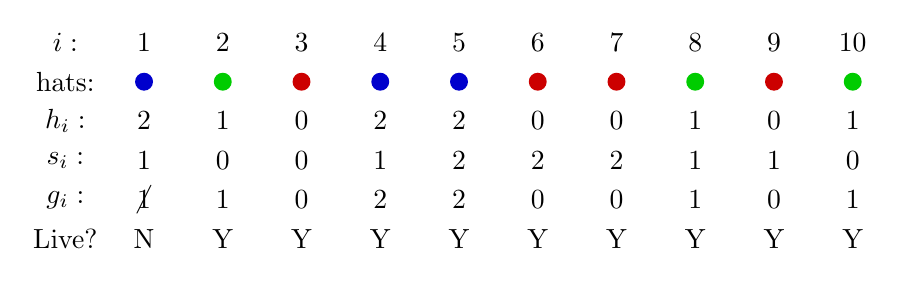
\begin{tikzpicture}[
    inner sep=2pt, %sets minimum size of a node
    bpt/.style={circle,draw=blue!80!black,fill=blue!80!black,thick,
        minimum size=2pt},
    gpt/.style={circle,draw=green!80!black,fill=green!80!black,thick,
        minimum size=2pt},
    rpt/.style={circle,draw=red!80!black,fill=red!80!black,thick,
        minimum size=2pt},
    kpt/.style={circle,draw=black,fill=black,thick,
        minimum size=2pt},
    >=angle 60,
    ]

    %Indices
    \node at (0,0.5) {$i:$};
    \node at (1,0.5) {1};
    \node at (2,0.5) {2};
    \node at (3,0.5) {3};
    \node at (4,0.5) {4};
    \node at (5,0.5) {5};
    \node at (6,0.5) {6};
    \node at (7,0.5) {7};
    \node at (8,0.5) {8};
    \node at (9,0.5) {9};
    \node at (10,0.5) {10};

    %hats
    \node at (0,0) {hats:};
    \node[bpt] at (1,0) {};
    \node[gpt] at (2,0) {};
    \node[rpt] at (3,0) {};
    \node[bpt] at (4,0) {};
    \node[bpt] at (5,0) {};
    \node[rpt] at (6,0) {};
    \node[rpt] at (7,0) {};
    \node[gpt] at (8,0) {};
    \node[rpt] at (9,0) {};
    \node[gpt] at (10,0) {};a

    %h_i
    \node at (0,-0.5) {$h_i:$};
    \node at (1,-0.5) {2};
    \node at (2,-0.5) {1};
    \node at (3,-0.5) {0};
    \node at (4,-0.5) {2};
    \node at (5,-0.5) {2};
    \node at (6,-0.5) {0};
    \node at (7,-0.5) {0};
    \node at (8,-0.5) {1};
    \node at (9,-0.5) {0};
    \node at (10,-0.5) {1};

    %s_i
    \node at (0,-1) {$s_i:$};
    \node at (1,-1) {1};
    \node at (2,-1) {0};
    \node at (3,-1) {0};
    \node at (4,-1) {1};
    \node at (5,-1) {2};
    \node at (6,-1) {2};
    \node at (7,-1) {2};
    \node at (8,-1) {1};
    \node at (9,-1) {1};
    \node at (10,-1) {0};

    %g_i
    \node at (0,-1.5) {$g_i:$};
    %\node at (1,-1.5) {1};
    \node at (1,-1.465) {$\cancel{1}$};
    \node at (2,-1.5) {1};
    \node at (3,-1.5) {0};
    \node at (4,-1.5) {2};
    \node at (5,-1.5) {2};
    \node at (6,-1.5) {0};
    \node at (7,-1.5) {0};
    \node at (8,-1.5) {1};
    \node at (9,-1.5) {0};
    \node at (10,-1.5) {1};
    
    %Live_i
    \node at (0,-2) {Live?};
    \node at (1,-2) {N};
    \node at (2,-2) {Y};
    \node at (3,-2) {Y};
    \node at (4,-2) {Y};
    \node at (5,-2) {Y};
    \node at (6,-2) {Y};
    \node at (7,-2) {Y};
    \node at (8,-2) {Y};
    \node at (9,-2) {Y};
    \node at (10,-2) {Y};

\end{tikzpicture}
\end{figure}
The top row shows the index number, $i$, where the left side is the back of 
the line facing to the right. Below this is the hat color, and the third 
row down is the number corresponding to each person's hat color, $h_i$. 
The equation each person needs says they all have to calculate $s_i$, 
the sum of the hat colors of all people in front of them, in $\mathbb{Z}_3$, 
which means then take the remainder when that number is divided by 3.
\begin{align*}
    s_1 &= (1+0+2+2+0+0+1+0+1)\%3 = 1 \\
    s_2 &= (0+2+2+0+0+1+0+1)\%3 = 0 \\
    s_3 &= (2+2+0+0+1+0+1)\%3 = 0 \\
    s_4 &= (2+0+0+1+0+1)\%3 = 1 \\
    s_5 &= (0+0+1+0+1)\%3 = 2 \\
    s_6 &= (0+1+0+1)\%3 = 2 \\
    s_7 &= (1+0+1)\%3 = 2 \\
    s_8 &= (0+1)\%3 = 1 \\
    s_9 &= (1)\%3 = 1 \\
    s_{10} &= 0 
\end{align*}
These are the values for each person for the fourth row, $s_i$, in the 
table above. 
The first person in line just guesses $g_1=s_1$, but everyone else must 
calculate more. Using the last equation above, everyone must 
subtract their sum, $s_i$ from 0 which cycles back around within $\mathbb{Z}_3$
(consult the Appendix).
\begin{align*}
    g_1 &= s_1 = 1 \\
    [0-s_2] &= [0-0] = 0 \\
    [0-s_3] &= [0-0] = 0 \\
    [0-s_4] &= [0-1] = 2 \\
    [0-s_5] &= [0-2] = 1 \\
    [0-s_6] &= [0-2] = 1 \\
    [0-s_7] &= [0-2] = 1 \\
    [0-s_8] &= [0-1] = 2 \\
    [0-s_9] &= [0-1] = 2 \\
    [0-s_{10}] &= [0-0] = 0 
\end{align*}
Now, everyone ahead of $i=1$ adds the first persons guess (in $\mathbb{Z}_3$, 
so apply the modulo-3 function).
\begin{align*}
    g_1 &= s_1 = 1 \\
    [0-s_2]+g_1 &= 0+1=1 \\
    [0-s_3]+g_1 &= 0+1=1 \\
    [0-s_4]+g_1 &= 2+1=0 \\
    [0-s_5]+g_1 &= 1+1=2 \\
    [0-s_6]+g_1 &= 1+1=2 \\
    [0-s_7]+g_1 &= 1+1=2 \\
    [0-s_8]+g_1 &= 2+1=0 \\
    [0-s_9]+g_1 &= 2+1=0 \\
    [0-s_{10}]+g_1 &= 0+1=1 
\end{align*}
Now, as each person shouts out their guess, people subtract the guesses 
of those after person 1 and before themselves (again, in $\mathbb{Z}_3$), 
the result is their own guess.
\begin{align*}
    g_1 &= s_1 = 1 \\
    \sum_{j=2}^{i-1}g_j
        =\sum_{j=2}^1g_j=0\qquad\qquad\Rightarrow\qquad\qquad g_2 &=
        [0-s_2]+g_1-\sum_{j=2}^1g_j = 1-0=1 \\
    \sum_{j=2}^2g_j=1\qquad\qquad \Rightarrow\qquad\qquad  g_3 &=
        [0-s_3]+g_1-\sum_{j=2}^2g_j  = 1-1=0 \\
    \sum_{j=2}^3g_j=1\qquad\qquad \Rightarrow\qquad\qquad  g_4 &=
        [0-s_4]+g_1-\sum_{j=2}^3g_j  = 0-1=2 \\
    \sum_{j=2}^4g_j=0\qquad\qquad \Rightarrow\qquad\qquad  g_5 &=
        [0-s_5]+g_1-\sum_{j=2}^4g_j  = 2-0=2 \\
    \sum_{j=2}^5g_j=2\qquad\qquad \Rightarrow\qquad\qquad  g_6 &=
        [0-s_6]+g_1-\sum_{j=2}^5g_j  = 2-2=0 \\
    \sum_{j=2}^6g_j=2\qquad\qquad \Rightarrow\qquad\qquad  g_7 &=
        [0-s_7]+g_1-\sum_{j=2}^6g_j  = 2-2=0 \\
    \sum_{j=2}^7g_j=2\qquad\qquad \Rightarrow\qquad\qquad  g_8 &=
        [0-s_8]+g_1-\sum_{j=2}^7g_j  = 0-2=1 \\
    \sum_{j=2}^8g_j=0\qquad\qquad \Rightarrow\qquad\qquad  g_9 &=
        [0-s_9]+g_1-\sum_{j=2}^8g_j  = 0-0=0 \\
    \sum_{j=2}^9g_j=0\qquad\qquad \Rightarrow\qquad\qquad  g_{10} &=
        [0-s_{10}]+g_1-\sum_{j=2}^9g_j  =1-0=1 
\end{align*}
The resultant guesses on the right hand side are exactly what was 
inserted into the fifth row, $g_i$, in the table above.
The first person in line guesses incorrectly, but everyone else lives. 
Remember you can tell if they survive by comparing $h_i$ to $g_i$.
This is strong evidence that the equation I derived and used to 
calculate these values is correct. Let's try another, without calculating 
every term, explicitly. I wrote a simple Python script to solve these.

\begin{figure}[H]
\centering
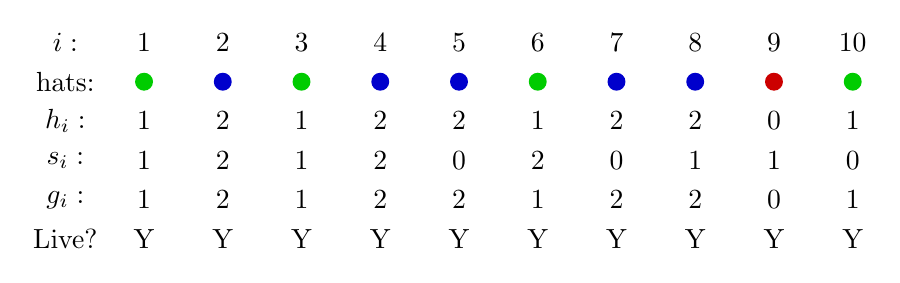
\begin{tikzpicture}[
    inner sep=2pt, %sets minimum size of a node
    bpt/.style={circle,draw=blue!80!black,fill=blue!80!black,thick,
        minimum size=2pt},
    gpt/.style={circle,draw=green!80!black,fill=green!80!black,thick,
        minimum size=2pt},
    rpt/.style={circle,draw=red!80!black,fill=red!80!black,thick,
        minimum size=2pt},
    kpt/.style={circle,draw=black,fill=black,thick,
        minimum size=2pt},
    >=angle 60,
    ]

    %Indices
    \node at (0,0.5) {$i:$};
    \node at (1,0.5) {1};
    \node at (2,0.5) {2};
    \node at (3,0.5) {3};
    \node at (4,0.5) {4};
    \node at (5,0.5) {5};
    \node at (6,0.5) {6};
    \node at (7,0.5) {7};
    \node at (8,0.5) {8};
    \node at (9,0.5) {9};
    \node at (10,0.5) {10};

    %hats
    \node at (0,0) {hats:};
    \node[gpt] at (1,0) {};
    \node[bpt] at (2,0) {};
    \node[gpt] at (3,0) {};
    \node[bpt] at (4,0) {};
    \node[bpt] at (5,0) {};
    \node[gpt] at (6,0) {};
    \node[bpt] at (7,0) {};
    \node[bpt] at (8,0) {};
    \node[rpt] at (9,0) {};
    \node[gpt] at (10,0) {};a

    %h_i
    \node at (0,-0.5) {$h_i:$};
    \node at (1,-0.5) {1};
    \node at (2,-0.5) {2};
    \node at (3,-0.5) {1};
    \node at (4,-0.5) {2};
    \node at (5,-0.5) {2};
    \node at (6,-0.5) {1};
    \node at (7,-0.5) {2};
    \node at (8,-0.5) {2};
    \node at (9,-0.5) {0};
    \node at (10,-0.5) {1};

    %s_i
    \node at (0,-1) {$s_i:$};
    \node at (1,-1) {1};
    \node at (2,-1) {2};
    \node at (3,-1) {1};
    \node at (4,-1) {2};
    \node at (5,-1) {0};
    \node at (6,-1) {2};
    \node at (7,-1) {0};
    \node at (8,-1) {1};
    \node at (9,-1) {1};
    \node at (10,-1) {0};

    %g_i
    \node at (0,-1.5) {$g_i:$};
    \node at (1,-1.5) {1};
    %\node at (1,-1.465) {$\cancel{1}$};
    \node at (2,-1.5) {2};
    \node at (3,-1.5) {1};
    \node at (4,-1.5) {2};
    \node at (5,-1.5) {2};
    \node at (6,-1.5) {1};
    \node at (7,-1.5) {2};
    \node at (8,-1.5) {2};
    \node at (9,-1.5) {0};
    \node at (10,-1.5) {1};

    %Live_i
    \node at (0,-2) {Live?};
    \node at (1,-2) {Y};
    \node at (2,-2) {Y};
    \node at (3,-2) {Y};
    \node at (4,-2) {Y};
    \node at (5,-2) {Y};
    \node at (6,-2) {Y};
    \node at (7,-2) {Y};
    \node at (8,-2) {Y};
    \node at (9,-2) {Y};
    \node at (10,-2) {Y};

\end{tikzpicture}
\end{figure}
In this particular example, everyone lives, even the first person in line. 
Let's try one last randomly generated example.
\begin{figure}[H]
\centering
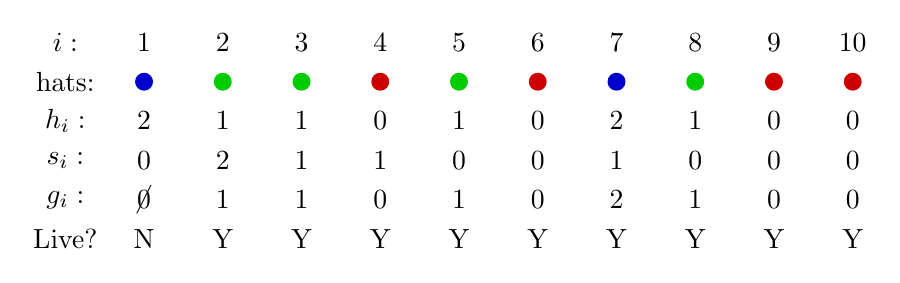
\begin{tikzpicture}[
    inner sep=2pt, %sets minimum size of a node
    bpt/.style={circle,draw=blue!80!black,fill=blue!80!black,thick,
        minimum size=2pt},
    gpt/.style={circle,draw=green!80!black,fill=green!80!black,thick,
        minimum size=2pt},
    rpt/.style={circle,draw=red!80!black,fill=red!80!black,thick,
        minimum size=2pt},
    kpt/.style={circle,draw=black,fill=black,thick,
        minimum size=2pt},
    >=angle 60,
    ]

    %Indices
    \node at (0,0.5) {$i:$};
    \node at (1,0.5) {1};
    \node at (2,0.5) {2};
    \node at (3,0.5) {3};
    \node at (4,0.5) {4};
    \node at (5,0.5) {5};
    \node at (6,0.5) {6};
    \node at (7,0.5) {7};
    \node at (8,0.5) {8};
    \node at (9,0.5) {9};
    \node at (10,0.5) {10};

    %hats
    \node at (0,0) {hats:};
    \node[bpt] at (1,0) {};
    \node[gpt] at (2,0) {};
    \node[gpt] at (3,0) {};
    \node[rpt] at (4,0) {};
    \node[gpt] at (5,0) {};
    \node[rpt] at (6,0) {};
    \node[bpt] at (7,0) {};
    \node[gpt] at (8,0) {};
    \node[rpt] at (9,0) {};
    \node[rpt] at (10,0) {};a

    %h_i
    \node at (0,-0.5) {$h_i:$};
    \node at (1,-0.5) {2};
    \node at (2,-0.5) {1};
    \node at (3,-0.5) {1};
    \node at (4,-0.5) {0};
    \node at (5,-0.5) {1};
    \node at (6,-0.5) {0};
    \node at (7,-0.5) {2};
    \node at (8,-0.5) {1};
    \node at (9,-0.5) {0};
    \node at (10,-0.5) {0};

    %s_i
    \node at (0,-1) {$s_i:$};
    \node at (1,-1) {0};
    \node at (2,-1) {2};
    \node at (3,-1) {1};
    \node at (4,-1) {1};
    \node at (5,-1) {0};
    \node at (6,-1) {0};
    \node at (7,-1) {1};
    \node at (8,-1) {0};
    \node at (9,-1) {0};
    \node at (10,-1) {0};

    %g_i
    \node at (0,-1.5) {$g_i:$};
    %\node at (1,-1.5) {0};
    \node at (1,-1.465) {$\cancel{0}$};
    \node at (2,-1.5) {1};
    \node at (3,-1.5) {1};
    \node at (4,-1.5) {0};
    \node at (5,-1.5) {1};
    \node at (6,-1.5) {0};
    \node at (7,-1.5) {2};
    \node at (8,-1.5) {1};
    \node at (9,-1.5) {0};
    \node at (10,-1.5) {0};

    %Live_i
    \node at (0,-2) {Live?};
    \node at (1,-2) {N};
    \node at (2,-2) {Y};
    \node at (3,-2) {Y};
    \node at (4,-2) {Y};
    \node at (5,-2) {Y};
    \node at (6,-2) {Y};
    \node at (7,-2) {Y};
    \node at (8,-2) {Y};
    \node at (9,-2) {Y};
    \node at (10,-2) {Y};

\end{tikzpicture}
\end{figure}
Again, the first person in line did not survive, but everyone else did. 
It appears the calculation is correct. It would yield $99\tfrac{1}{3}$ 
of the 100 people alive, assuming everything is done correctly. 
But what if someone makes a mistake or gets killed arbitrarily?

\subsection{Mistake or Malevolent Caprice}

What if someone made a mistake, or perhaps if the warden randomly orders 
people to be killed. In reality, if the warden doesn't say something, 
you wouldn't really know which is which if someone got killed. The people in 
back would know, but they can't communicate that to the people in front. 
Even if the warden does say something, you don't know if they're telling 
the truth. This could be a good application for probability theory.

If someone other than in the very back gets shot, the next person could 
theoretically choose to pursue one of two general approaches:
\begin{itemize}
    \item Start over from the beginning, as if they were the one in the 
    back, giving them a 1/3 chance of surviving.
    \item Try to take information from the event, the previous person 
    getting shot, to improve their chance of surviving.
\end{itemize}
In reality, considering this is a thought experiment to see 
which choice is best. What people do 
needs to be agreed upon by everyone in the 24 hours prior to the line up. 
Otherwise, the people in the front might not know how to proceed.

Let's investigate the second choice, to see if someone could pull 
some information from the event, that someone got shot. 
If it was a simple error on the participant's part, then it is one of 
the other two hats. The next person could then assume one and perform 
their calculation as if their guess about the previous hat was correct. 
They would have a 50\% chance of surviving, conditioned on it being 
just a mistake. 

But it might not just be a mistake. If it is a malicious whim of the warden 
or guard, then the hat they called out was correct. If that was true, 
the next person would have a 100\% chance of getting their hat correct 
(conditioned on them not making a mistake, too). Which one is more 
likely? Is a participant making a mistake more likely than the Nazi guard 
being maliciously capricious? There's a decent chance of someone making 
a mistake, with how difficult the calculation is. But these are Nazi's. 
They could very conceivably do this. 

Let's assume maximum ignorance and 
say there's a 50\% chance the shooting was caused by a mistake and a 50\% 
chance it was malice by the guard or warden. We need to pick a method: assume 
it is a mistake and pick one of the other two hats, or assume it is malice and 
choose your hat as if the previous person got their hat correct.
\begin{align*}
    P(live|pick\_mistake) = &P(live|mistake\,and\,pick\_mistake)P(mistake) \\
        &+ P(live|malice\,and\,pick\_mistake)P(malice) \\
    &= 0.5\cdot0.5 + 0.0\cdot0.5 \\
    P(live|pick\_mistake) = &0.25 \\
    P(live|pick\_malice) = &P(live|mistake\,and\,pick\_malice)P(mistake) \\
        &+ P(live|malice\,and\,pick\_malice)P(malice) \\
    = &0.0\cdot0.5 + 1.0\cdot0.5 \\
    P(live|pick\_malice) = &0.5
\end{align*}
This uses conditional and marginal probabilities, and note that if what you 
choose ($pick\_mistake$ or $pick\_malice$) does not match what the actual 
cause of the shooting was ($mistake$ or $malice$), then there is a zero chance 
of living, because they lead you to shout the wrong hat color.
Here, it seems that assuming it was malice causing the shot is the best choice.
But a 50\% chance may not be the real odds of the shot being caused by 
a mistake. What is the cutoff that would maximize the chance of survival for 
each method? Let $p = P(mistake)$ be a variable, we optimize for, and 
$(1-p) = P(malice)$.
\begin{align*}
    P(live|pick\_mistake) =&P(live|mistake\,and\,pick\_mistake)p \\
        &+ P(live|malice\,and\,pick\_mistake)(1-p) \\
    =&0.5\cdot p + 0.0\cdot(1-p) \\
    P(live|pick\_mistake) = &0.5p \\
    P(live|pick\_malice) = &P(live|mistake\,and\,pick\_malice)p \\
        &+ P(live|malice\,and\,pick\_malice)(1-p) \\
    = &0.0\cdot p + 1.0\cdot(1-p) \\
    P(live|pick\_malice) = &1-p
\end{align*}
If there's a 67\% chance that someone being shot is caused by a mistake 
on that person's part, then the chance of living by assuming it was 
a mistake drops to 33\%, matching the odds of living by just starting over 
as if you're in the back and guessing. In this same event, the odds of 
living by guessing it was malice drops to 33\% as well. The following 
graph shows the different choices. The optimum solution, the one that 
gets you the best chance of living, depends on how likely it is 
a shooting (after the first person) is caused by a mistake.
\begin{figure}[H]
\centering
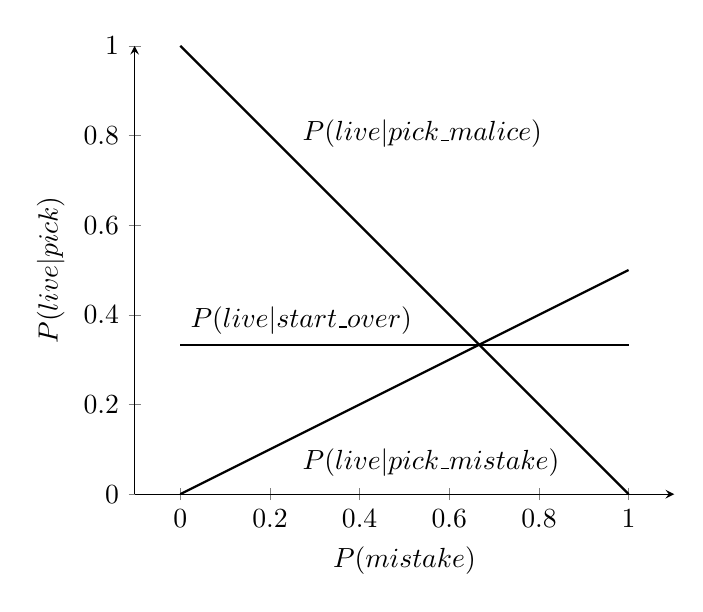
\begin{tikzpicture}
    \begin{axis}[
        axis equal,
        axis x line=bottom,
        axis y line=left,
        xmin=0,xmax=1,
        ymin=0,ymax=1,
        xlabel={$P(mistake)$},
        ylabel={$P(live|pick)$},
        ]

        \addplot[black, thick, variable=\p,
            domain=0:1,smooth,samples=20]
            (\p,{0.5*\p})
            node[pos=0.25,below right] {$P(live|pick\_mistake)$};
        
        \addplot[black, thick, variable=\p,
            domain=0:1,smooth,samples=20]
            (\p,{1-\p})
            node[pos=0.25,above right] {$P(live|pick\_malice)$};
        
        \addplot[black, thick, variable=\p,
            domain=0:1,smooth,samples=20]
            (\p,0.333)
            node[pos=0.0,above right] {$P(live|start\_over)$};

    \end{axis}
\end{tikzpicture}
\end{figure}
Choosing that the warden or guard was malicious gives the best chance of 
survival, for the widest range of $P(mistake)$. Only if this is greater 
than a 67\% chance does it become best to assume they made a mistake. It 
is never best to start over in the event that someone other than the first 
person was shot. It is best just to use the guess of the previous person 
as if it was correct, unless after multiple test runs, you find a very 
high error rate. 

Imagine the worst case scenario, many people get killed in a row despite 
all agreeing to assume that malice is causing everyone to get shot. 
It seems this is consistent with extreme malice (plausible for Nazi's) and 
extremely bad math (less likely). It still seems that 
assuming malice is best, but 
then again, you're probably going to get shot anyway, so you might as well 
try to make a run for it if many people in a row start to get shot. 
How many in a row need to get shot for this to be best? It depends on the 
odds of escape, which I would guess is really unlikely. So it would need to be 
several, especially since you running will likely result in many others 
getting killed. But more precisely how many, how likely it is to escape, 
is beyond the scope of this brain teaser.

\newpage

\subsection{Appendix: Basic Properties of $\mathbb{Z}_n$ and the Modulus Function}

Incrementing through the cyclic group 
$\mathbb Z_n$ can be visualized by the following example diagram:
\begin{figure}[H]
\centering
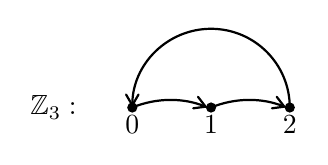
\begin{tikzpicture}[
    scale=0.5,
    inner sep=1pt, %sets minimum size of a node
    bpt/.style={circle,draw=blue!50,fill=blue!50,thick,
        minimum size=1pt},
    gpt/.style={circle,draw=green!50,fill=green!50,thick,
        minimum size=1pt},
    rpt/.style={circle,draw=red!50,fill=red!50,thick,
        minimum size=1pt},
    kpt/.style={circle,draw=black,fill=black,thick,
        minimum size=1pt},
    >=angle 60,
    ]
    \node at (-2,0) {$\mathbb{Z}_3:$};
    %\node at (-2,1) [label={above:$\mathbb{Z}_3:$}] {};
    \node[kpt] (a) at (0,0) [label={below:0}] {};
    \node[kpt] (b) at (2,0) [label={below:1}] {};
    \node[kpt] (c) at (4,0) [label={below:2}] {};
    \draw[thick,black,->] (a)
        arc[start angle=112.5,delta angle=-45,radius=2.5]
        ;
    \draw[thick,black,->] (b)
        arc[start angle=112.5,delta angle=-45,radius=2.5]
        ;
    \draw[thick,black,->] (c)
        arc[start angle=0,delta angle=180,radius=2]
        ;
\end{tikzpicture}
\hspace{1in}
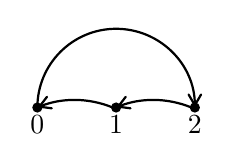
\begin{tikzpicture}[
    scale=0.5,
    inner sep=1pt, %sets minimum size of a node
    bpt/.style={circle,draw=blue!50,fill=blue!50,thick,
        minimum size=1pt},
    gpt/.style={circle,draw=green!50,fill=green!50,thick,
        minimum size=1pt},
    rpt/.style={circle,draw=red!50,fill=red!50,thick,
        minimum size=1pt},
    kpt/.style={circle,draw=black,fill=black,thick,
        minimum size=1pt},
    >=angle 60,
    ]
    \node[kpt] (a) at (0,0) [label={below:0}] {};
    \node[kpt] (b) at (2,0) [label={below:1}] {};
    \node[kpt] (c) at (4,0) [label={below:2}] {};
    \draw[thick,black,<-] (a)
        arc[start angle=112.5,delta angle=-45,radius=2.5]
        ;
    \draw[thick,black,<-] (b)
        arc[start angle=112.5,delta angle=-45,radius=2.5]
        ;
    \draw[thick,black,<-] (c)
        arc[start angle=0,delta angle=180,radius=2]
        ;
\end{tikzpicture}
\end{figure}

Doing addition and subtraction in $\mathbb{Z}_n$ is equivalent to 
doing the operations in the ordinary integers, $\mathbb{Z}$,
followed by taking the remainder when dividing by 
$n$, which means applying the modulo-$n$ function to the result of the addition 
or subtraction. There is one caveat, 
which is dealing with negative numbers. I'll get to that. The following 
shows this equivalence relationship I just mentioned.
\begin{equation}
    (a+b+c)_{\mathbb{Z}_n}=(a+b+c)_{\mathbb{Z}}\%n \tag{$a,b,c\geq 0$}
\end{equation}
Cycling through the integers in the diagram above, argues
you can apply the modulus function repeatedly 
and your answer will always remain in $\mathbb{Z}_n$, giving you one unique 
answer. This has to do with the group structure of $\mathbb{Z}_n$. 
\begin{align}
    (a+b+c+d)\% n &= (((a+b)\% n + c)\%n + d)\% n \notag \\
    \notag \\
    (2+2+1+2)\% 3 &= (((2+2)\%3 + 1)\% 3 + 2)\% 3 \tag{Example: $n=3$}\\
    7\% 3 &= ((4\%3+1)\%3+ 2)\% 3 \notag \\
    1 &= ((1+1)\%3+ 2)\% 3 \notag \\
    1 &= (2\%3+ 2)\% 3 \notag \\
    1 &= (2 + 2)\% 3 \notag \\
    1 &= 4\% 3 \notag \\
    1 &= 1 \notag 
\end{align}
Negative numbers in $\mathbb{Z}_n$ wrap around to $n$, as you would expect 
by looking at the diagram at the beginning of this Appendix. The following 
demonstrates this by showing a negative number is just 0 minus its absolute 
value.
\begin{align}
    -m &= 0 - m \notag \\
    0 &= (pn)\%n \tag{Let $p\in\mathbb{Z}$ and $pn > m$}\\
    -m_{\mathbb{Z}_n} &= (0 - m)\%n \notag \\
    &= ((pn)\%n - m)\%n \notag \\
    &= (pn-m)\%n \notag \\
    \notag \\
    -1_{\mathbb{Z}_3} &= (0-1)\%3 \tag{Example: $n=3$} \\
    &= (3\%3-1)\%3 \notag \\
    &= (3-1)\%3 \notag \\
    &= 2\%3 \notag \\
    &= 2 \notag
\end{align}
These relationships are enough to understand algebra in $\mathbb{Z}_n$.

\end{document}
